%% LyX 2.3.5.2 created this file.  For more info, see http://www.lyx.org/.
%% Do not edit unless you really know what you are doing.
\documentclass[english]{article}
\PassOptionsToPackage{natbib=true}{biblatex}
\renewcommand{\rmdefault}{futs}
\usepackage[T1]{fontenc}
\usepackage[utf8]{inputenc}
\usepackage{geometry}
\geometry{verbose,tmargin=2cm,bmargin=2cm,lmargin=2cm,rmargin=2cm}
\usepackage{babel}
\usepackage{amsmath}
\usepackage{amssymb}
\usepackage{graphicx}
\usepackage[unicode=true]
 {hyperref}

\makeatletter
%%%%%%%%%%%%%%%%%%%%%%%%%%%%%% User specified LaTeX commands.
%\usepackage[style=numeric,backend=biber,maxbibnames=99]{biblatex}
\usepackage{hyperref}

\AtBeginDocument{
  \def\labelitemii{\(\ast\)}
  \def\labelitemiii{\(\star\)}
}

\makeatother

\usepackage[style=authoryear,maxbibnames=99]{biblatex}
\addbibresource{papers.bib}
\begin{document}
\title{Paper summaries}

\maketitle
\global\long\def\vec#1{\text{\textbf{#1}}}%


\section{\protect\href{https://docs.google.com/presentation/d/1m4Z3RJDueaKMvCO-cb_Ia51nTW6-OSE9hXVPy1l1-_I/edit?usp=sharing}{On the Automatic Generation of Medical Imaging Reports}
\citep{baoyu_jing2018}}

\subsection{Introduction}

The reading and interpretation of medical images are usually conducted
by specialized medical professionals. Report writing can be error-prone
for inexperienced physicians, and time-consuming and tedious for experienced
physicians. \\
Several challenges need to be addressed:
\begin{enumerate}
\item A complete report consists of multiple heterogeneous sources of information
\item Localize image regions and attach the right description to them 
\item Descriptions in reports are usually long, with multiple sentences
\end{enumerate}
The proposed solutions are:
\begin{enumerate}
\item A \textbf{multi-task learning framework} for simultaneous prediction
of tags and text generation
\item A \textbf{Co-attention mechanism: }simultaneous attention to images
and predicted tags; explores synergistic effects of visual and semantic
information 
\item A \textbf{Hierarchical LSTM: }Leverages compositional nature of reports:
first generates high-level topics, then fine-grained descriptions
from each one
\end{enumerate}
\begin{figure}
\begin{centering}
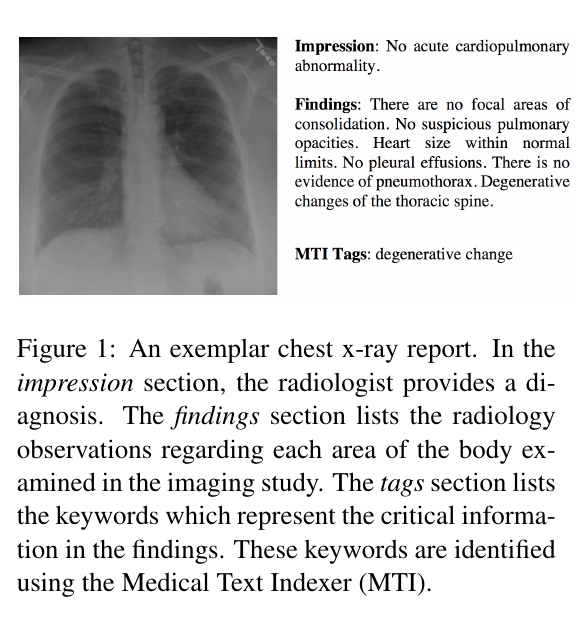
\includegraphics[scale=0.5]{images/baoyu_jing_report}
\par\end{centering}
\caption{Sample report from IU X-ray}

\end{figure}


\subsection{Methods and Architecture}

An image is divided into regions, and a CNN encoder is used to learn
visual features for these patches. These features are fed into a \emph{multi-label
classifier}, from which tags are predicted. These tags are transformed
into \emph{semantic feature vectors }by a custom embedding. Both visual
and semantic features are fed into the co-attention module, which
produces a combined \emph{context vector, }which \textbf{simultaneously
captures the visual and semantic information of this image.} 

The decoding and caption generation process is performed by the hierarchical
LSTM, which leverages the compositional structure of a medical report
(each sentence focusing on one specific topic). The \emph{sentence
LSTM}, using the context vector, first generates a sequence of high-level
topic vectors representing sentences. Each one is passed to the \emph{word
LSTM,} which then generates a sentence for each topic vector. The
number of sentences or topic vectors to be generated is regulated
by the \emph{stop control}.

\begin{figure}
\begin{centering}
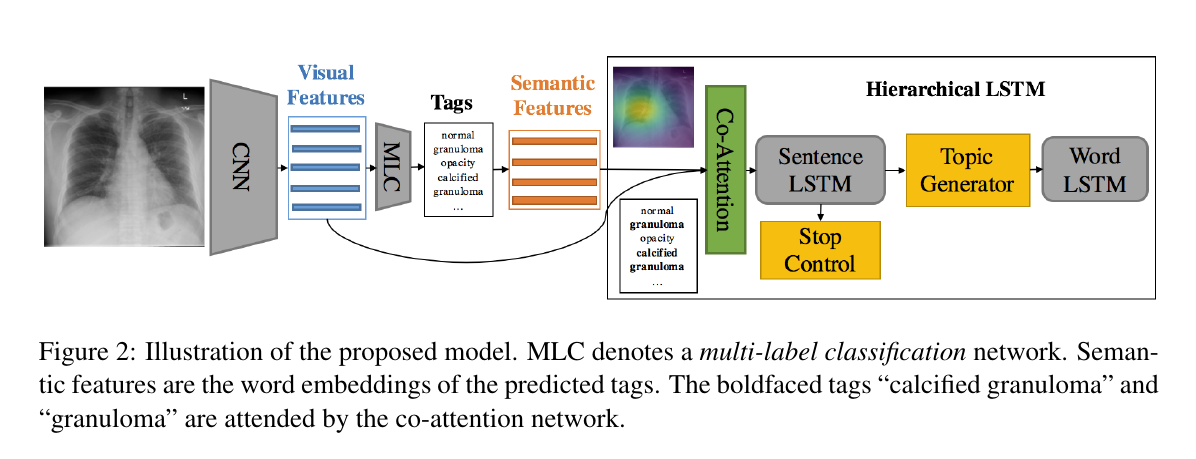
\includegraphics[scale=0.5]{images/baoyu_jing_architecture}
\par\end{centering}
\caption{Architecture}
\end{figure}


\subsubsection{Tag prediction}

This is treated as a multi-label classification task. Given an image
$I$, visual features $\left\{ \boldsymbol{v}_{n}\right\} _{n=1}^{N}\in\mathbb{R}^{D}$
are extracted from the CNN encoder, and fed to a \emph{multi-label
classification }(MLC) network, which then generates a probability
distribution over the $L$ tags
\[
\boldsymbol{p}_{I,\text{pred}}\left(\boldsymbol{l}_{i}=1\;|\;\left\{ \boldsymbol{v}_{n}\right\} _{n=1}^{N}\right)\propto\exp\left(\text{MLC}_{i}\left(\left\{ \boldsymbol{v}_{n}\right\} _{n=1}^{N}\right)\right)
\]
\\
where $\boldsymbol{l}\in\mathbb{R}^{L}$ is a binary tag vector, each
component representing the presence or absence of the corresponding
tag.\\
Finally, the embeddings of the $M$ most likely tags $\left\{ \boldsymbol{a}_{m}\right\} _{m=1}^{M}$
are used as \textbf{semantic features. }

\subsubsection{Co-Attention}

Visual attention does not provide sufficient high-level semantic information,
which the tags can always provide. A co-attention mechanism can simultaneously
attend to visual and semantic modalities.

In the sentence LSTM at time step $s$, the joint context vector \textbf{$\text{\textbf{ctx}}^{(s)}\in\mathbb{R}^{C}$
}is generated by a co-attention network $f_{\text{co-att}}\left(\left\{ \boldsymbol{v}_{n}\right\} _{n=1}^{N},\left\{ \boldsymbol{a}_{m}\right\} _{m=1}^{M},\boldsymbol{h}_{\text{sent}}^{(s-1)}\right)$,
with $\boldsymbol{h}_{\text{sent}}^{(s-1)}\in\mathbb{R}^{H}$ being
the previous hidden state. The co-attention network $f_{\text{co-att}}$
uses a single feedforward layer to compute separate soft visual and
semantic attentions
\begin{align*}
\alpha_{\vec v,n} & \propto\exp\left(\vec W_{\vec v_{\text{att}}}\vec v_{n}+\vec W_{\vec v,\vec h}\vec h_{\text{sent}}^{(s-1)}\right)\\
\alpha_{\vec a,m} & \propto\exp\left(\vec W_{\vec a_{\text{att}}}\vec a_{m}+\vec W_{\vec a,\vec h}\vec h_{\text{sent}}^{(s-1)}\right)
\end{align*}
\\
The visual and semantic context vectors 
\begin{align*}
\vec v_{\text{att}}^{(s)} & =\sum_{n=1}^{N}\alpha_{\vec v,n}\vec v_{n}\\
\vec a_{\text{att}}^{(s)} & =\sum_{m=1}^{M}\alpha_{\vec a,m}\vec a_{m}
\end{align*}
\\
These context vector may be combined by concatenation followed by
a fully connected layer:

\[
\vec{ctx}^{(s)}=\vec W_{\text{fc}}\left[\vec v_{\text{att}}^{(s)};\vec a_{\text{att}}^{(s)}\right]
\]


\subsubsection{Sentence LSTM}

A single LSTM layer whose input is the joint context vector $\vec{ctx}^{(s)}$
and generates a topic vector $\vec t\in\mathbb{R}^{K}$as long as
the stop control allows it to. 

\paragraph{Topic generator}

Deep output layer (LSTM + multi-layer feedforward) 
\[
\vec t^{(s)}=\tanh\left(\vec W_{\vec t,\vec h}\vec h_{\text{sent}}^{(s)}+\vec W_{\vec t,\vec{ctx}}\vec{ctx}^{(s)}\right)
\]


\paragraph{Stop control }

Deep output layer for the continuation of the sentence LSTM. The layer
takes the previous and current hidden states and produces a distribution
over $\left\{ \text{STOP}=1,\text{CONTINUE}=0\right\} $
\begin{align*}
p\left(\text{STOP}\;|\;\vec h_{\text{sent}}^{(s-1)},\vec h_{\text{sent}}^{(s)}\right) & \propto\\
 & \exp\left\{ \text{\ensuremath{\vec W_{\text{stop}}\tanh\left(\vec W_{\text{stop},s-1}\vec h_{\text{sent}}^{(s-1)}+\vec W_{\text{stop},s-1}\vec h_{\text{sent}}^{(s)}\right)}}\right\} 
\end{align*}
\\
This stopping probability is then compared with a predefined threshold.

\subsubsection{Word LSTM}

\printbibliography

\end{document}
